\documentclass[protokol.tex]{subfiles}
\begin{document}
\begin{comment}
\begin{table}[H] \label{tab:podminky}
\centering
\setlength{\tabcolsep}{10pt}
\begin{tabular}{ccc}                                                    \toprule
Teplota                 &   Tlak                    &   Vlhkost     \\
$[\si{\degreeCelsius}]$ &   $[\si{\hecto\pascal}]$  &   [\% RH]     \\  \midrule
25,3                    &   984,5                   &   29,8        \\  \bottomrule
\end{tabular}
\caption{Podmínky měření}
\end{table}

\begin{figure}[H]
\centering
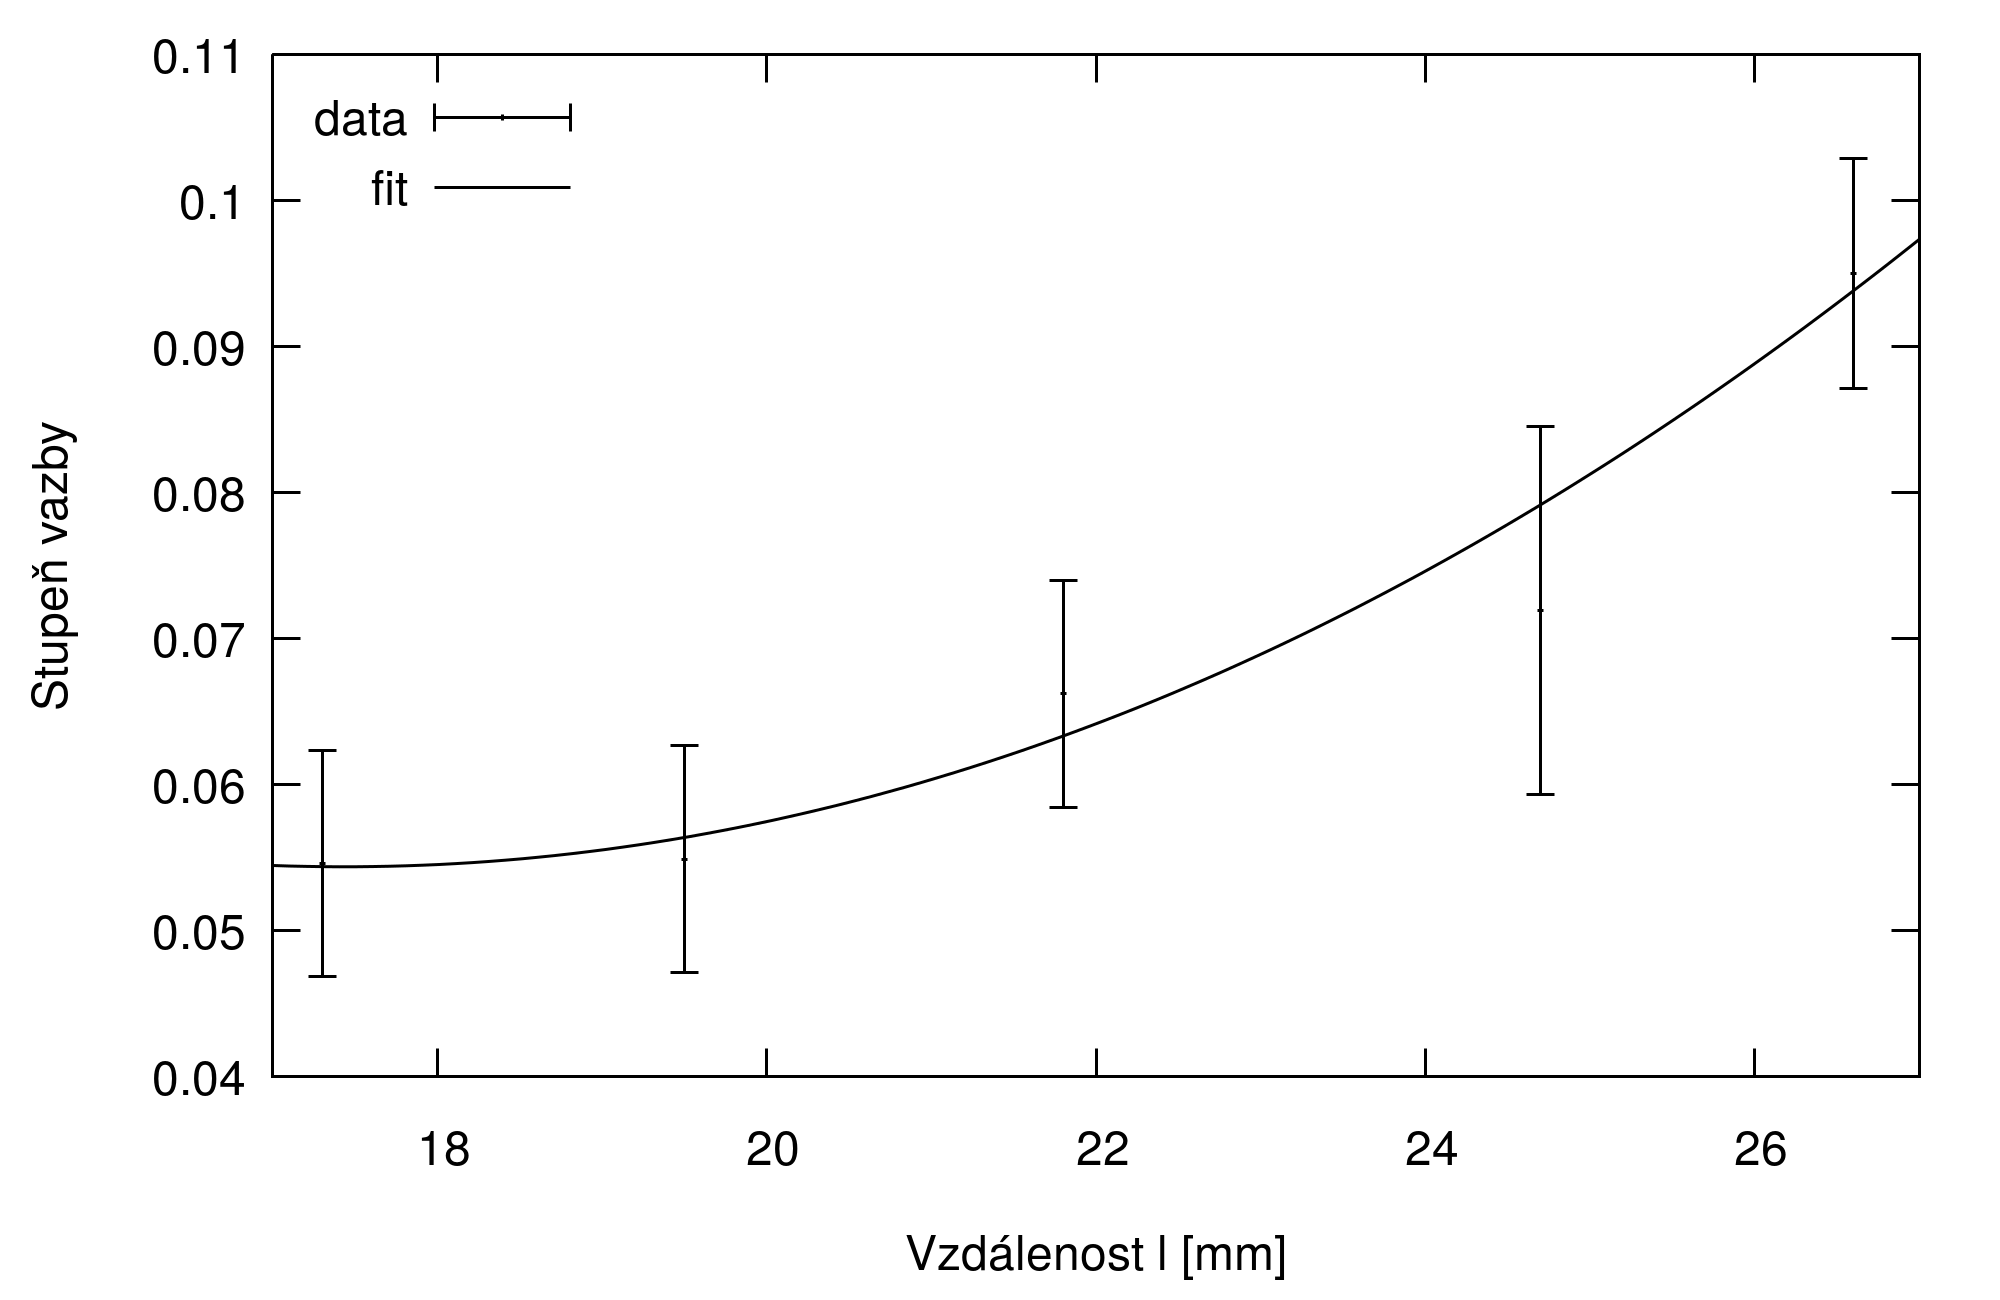
\includegraphics[resolution=350]{plot/graf}
\caption{Graf závislosti napětí na relativním prodloužení}
\end{figure}
\end{comment}

Měření probíhalo při teplotě $24.5 \si{\celsius}$.

Délka drátu (vnitřní šířka rámečku) byla měřena posuvným měřidlem.
$$ l = (1.964 \pm 0.002) \times \num{e-2} \ \si{\metre} $$

Průměr drátu byl měřen mikrometrem na třech místech.
$$ r = (0.60 \pm 0.01) \times \num{e-3} \ \si{\metre} $$

V následující tabulce jsou uvedeny rozdíly hodnot naměřených torzními váhami $\Delta m$ a hodnoty $P_0$. Pro výpočty je využita přibližná hodnota tíhového zrychlení $g = 9.81 \si{\metre\per\second\squared}$.

\begin{table}[H] \label{tab:tab}
\centering
\setlength{\tabcolsep}{15pt}
\begin{tabular}{ccc}                                                                    \toprule
$c [\si{\percent}]$   &   $\Delta m [\si{\milli\gram}]$ &   $P_0 [\si{\newton}]$    \\  \midrule
100                   &   117                           &   0.00115                 \\
50                    &   151                           &   0.00148                 \\
25                    &   190                           &   0.00186                 \\
12.5                  &   230                           &   0.00226                 \\
6.25                  &   253                           &   0.00248                 \\
3.125                 &   255                           &   0.00250                 \\
1.5625                &   264                           &   0.00259                 \\
0                     &   297                           &   0.00291                 \\  \bottomrule
\end{tabular}
\caption{$\Delta m$ a $P_0$ v závislosti na koncentraci $c$}
\end{table}

\newpage

Následující graf zachycuje závislost povrchového napětí počítaného pomocí \eqref{eq:sigma}. Lineární regrese byla provedena pomocí křivky $y = ae^{bx} + c$.
\begin{figure}[H]
\centering
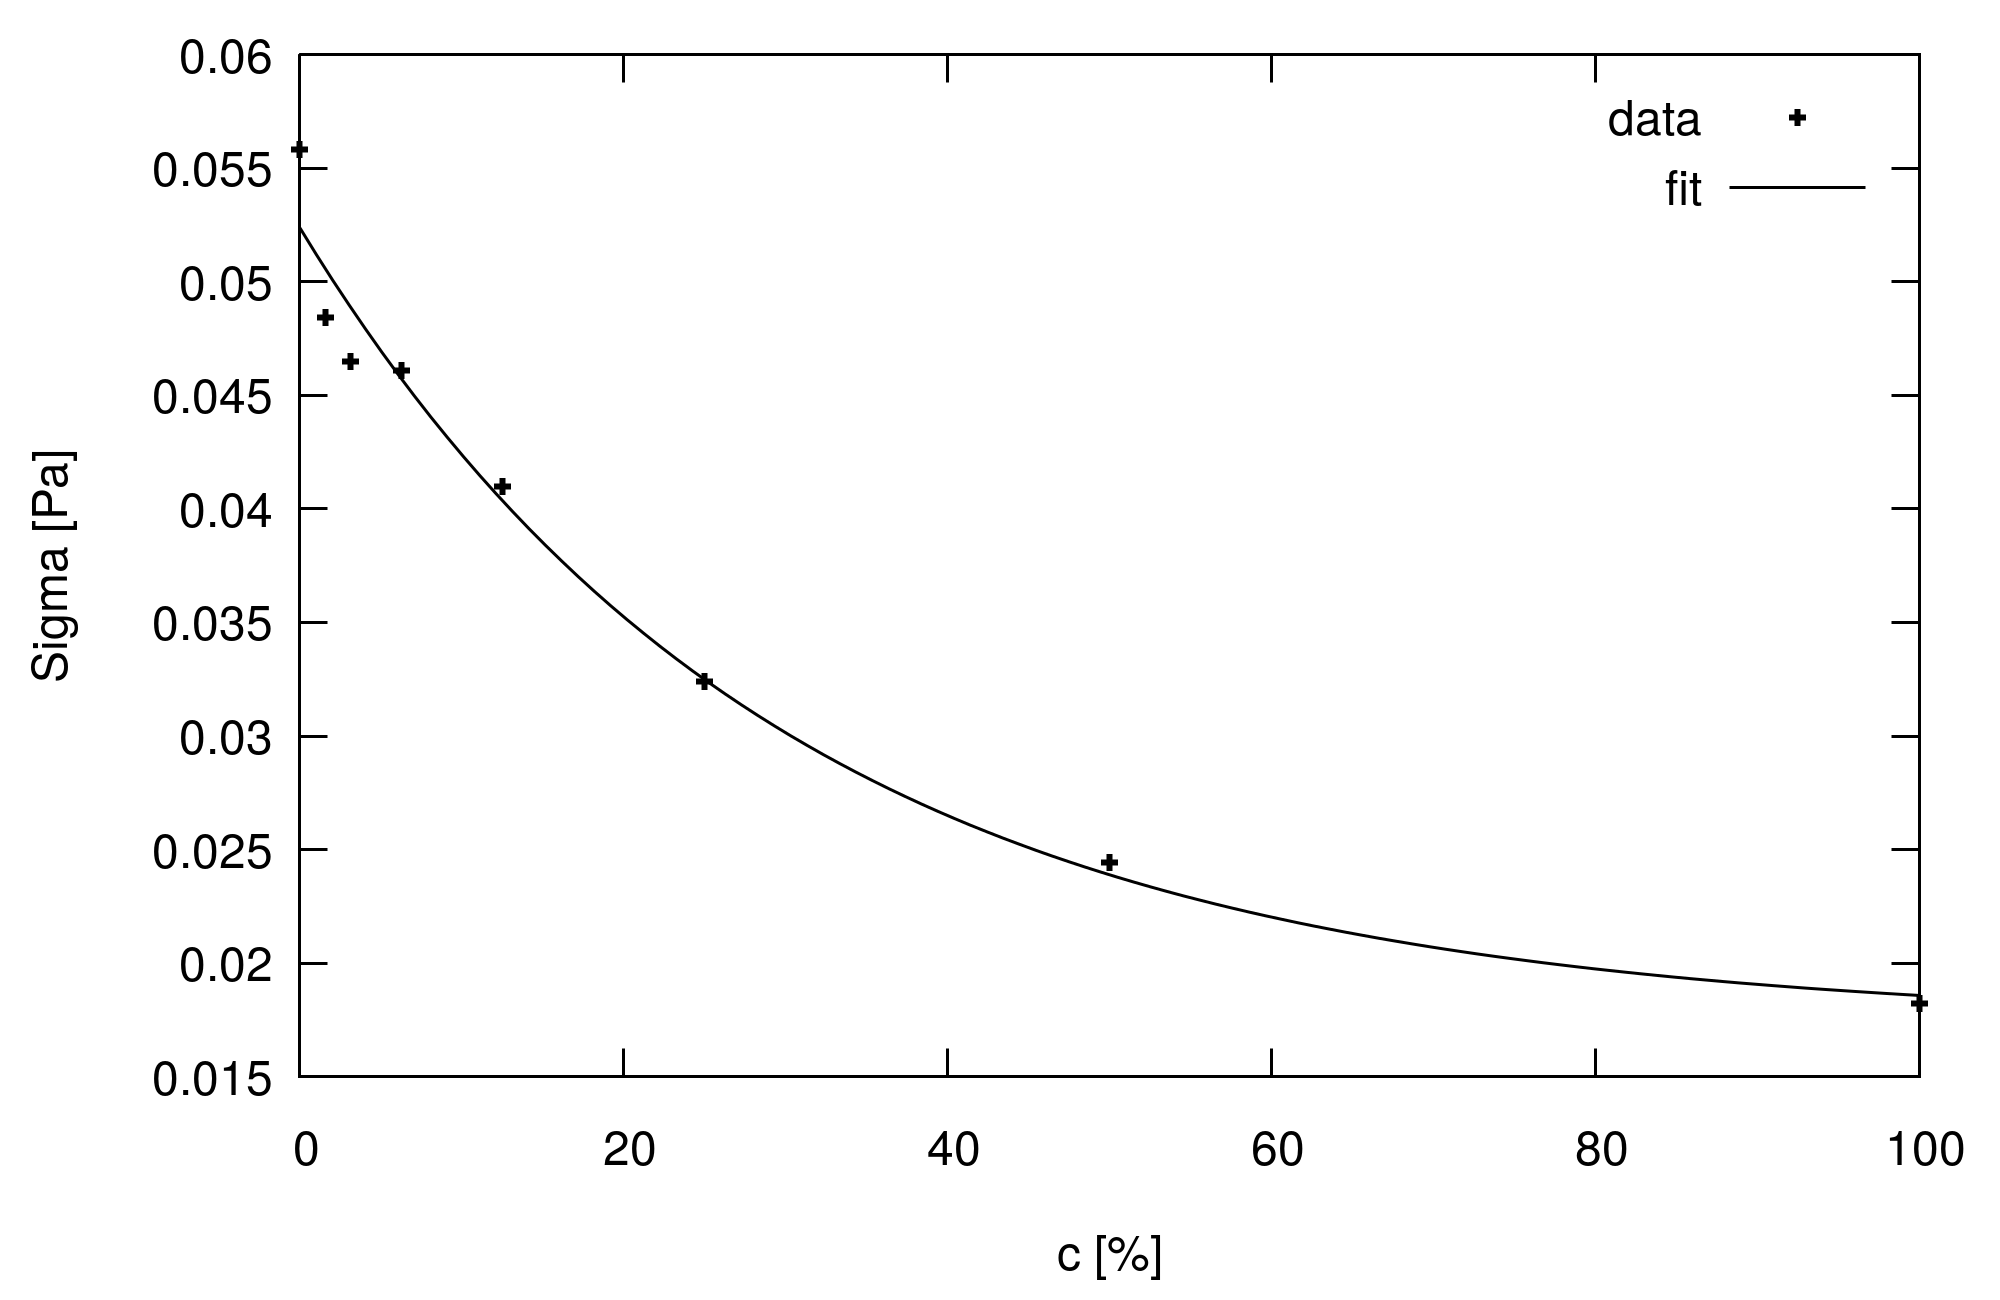
\includegraphics[resolution=350]{plot/out}
\caption{Graf závislosti povrchového napětí na koncentraci}
\end{figure}

\begin{table}[H] \label{tab:parametry}
\centering
\setlength{\tabcolsep}{10pt}
\begin{tabular}{cccc}                               \toprule
            &   a       &   b       &   c       \\  \midrule
hodnota     &   0.035   &   -0.034  &   0.007   \\
chyba       &   0.003   &   0.017   &   0.002   \\  \bottomrule
\end{tabular}
\caption{Parametry lineární regrese}
\end{table}
\end{document}
